\section{Startbildschirm}
\autorbeginn{Marcel}
\label{sec:ui-startbildschirm}

Zu Beginn des Unternehmensplanspiels „StarGreg“ öffnet sich ein Startbildschirm. Hierbei muss der Spieler, sein Unternehmen einrichten und somit ein neues Spiel generieren lassen. Zur Einrichtung des Unternehmens wird ein Unternehmensname erfordert, der nach belieben festgelegt werden kann. Hierzu steht ein Textfeld oberhalb des sogenannten „CoverFlows“ bereit. Neben dem Unternehmensnamen muss sich der Spieler auch für ein Firmenlogo entscheiden. Hierfür steht ein Coverflow bereit, das verschiedene Bilder enthält.
 
Nach getätigter Eingabe des Unternehmensnamen und der Auswahl des Firmenlogos bestätigt der Spieler seine Eingaben durch drücken des rot hinterlegten „StarGreg Starten“ Buttons. Durch diesen Button wird der UseCase „Unternehmen einrichten“ ausgelöst. Infolgedessen wird das Unternehmensplanspiel gestartet und der Spieler gelangt zur nächsten Benutzeroberfläche, der Spielübersicht. (\ref{img:ui-startbildschirm})

\begin{figure}[h]
  \centering
  \fbox{
    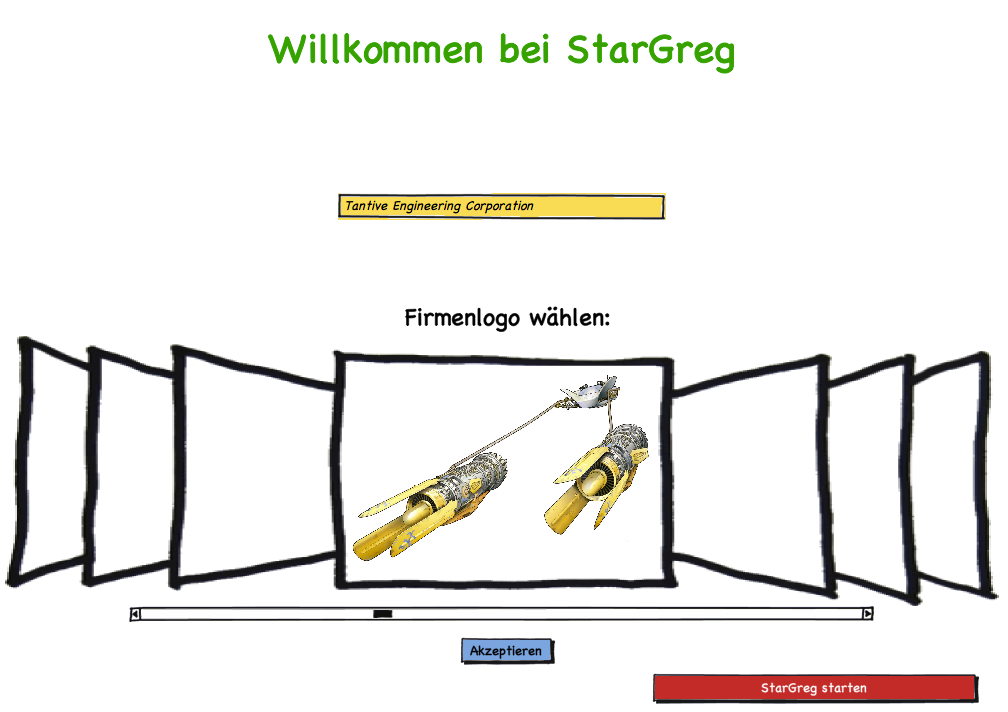
\includegraphics[width=0.9\textwidth]{40_UI/15_Startbildschirm/Startbildschirm.png}
  }
  \caption{Startbildschirm}
  \label{img:ui-startbildschirm}
\end{figure}

\autorende{}
 